\documentclass[1p]{elsarticle_modified}
%\bibliographystyle{elsarticle-num}

%\usepackage[colorlinks]{hyperref}
%\usepackage{abbrmath_seonhwa} %\Abb, \Ascr, \Acal ,\Abf, \Afrak
\usepackage{amsfonts}
\usepackage{amssymb}
\usepackage{amsmath}
\usepackage{amsthm}
\usepackage{scalefnt}
\usepackage{amsbsy}
\usepackage{kotex}
\usepackage{caption}
\usepackage{subfig}
\usepackage{color}
\usepackage{graphicx}
\usepackage{xcolor} %% white, black, red, green, blue, cyan, magenta, yellow
\usepackage{float}
\usepackage{setspace}
\usepackage{hyperref}

\usepackage{tikz}
\usetikzlibrary{arrows}

\usepackage{multirow}
\usepackage{array} % fixed length table
\usepackage{hhline}

%%%%%%%%%%%%%%%%%%%%%
\makeatletter
\renewcommand*\env@matrix[1][\arraystretch]{%
	\edef\arraystretch{#1}%
	\hskip -\arraycolsep
	\let\@ifnextchar\new@ifnextchar
	\array{*\c@MaxMatrixCols c}}
\makeatother %https://tex.stackexchange.com/questions/14071/how-can-i-increase-the-line-spacing-in-a-matrix
%%%%%%%%%%%%%%%

\usepackage[normalem]{ulem}

\newcommand{\msout}[1]{\ifmmode\text{\sout{\ensuremath{#1}}}\else\sout{#1}\fi}
%SOURCE: \msout is \stkout macro in https://tex.stackexchange.com/questions/20609/strikeout-in-math-mode

\newcommand{\cancel}[1]{
	\ifmmode
	{\color{red}\msout{#1}}
	\else
	{\color{red}\sout{#1}}
	\fi
}

\newcommand{\add}[1]{
	{\color{blue}\uwave{#1}}
}

\newcommand{\replace}[2]{
	\ifmmode
	{\color{red}\msout{#1}}{\color{blue}\uwave{#2}}
	\else
	{\color{red}\sout{#1}}{\color{blue}\uwave{#2}}
	\fi
}

\newcommand{\Sol}{\mathcal{S}} %segment
\newcommand{\D}{D} %diagram
\newcommand{\A}{\mathcal{A}} %arc


%%%%%%%%%%%%%%%%%%%%%%%%%%%%%5 test

\def\sl{\operatorname{\textup{SL}}(2,\Cbb)}
\def\psl{\operatorname{\textup{PSL}}(2,\Cbb)}
\def\quan{\mkern 1mu \triangleright \mkern 1mu}

\theoremstyle{definition}
\newtheorem{thm}{Theorem}[section]
\newtheorem{prop}[thm]{Proposition}
\newtheorem{lem}[thm]{Lemma}
\newtheorem{ques}[thm]{Question}
\newtheorem{cor}[thm]{Corollary}
\newtheorem{defn}[thm]{Definition}
\newtheorem{exam}[thm]{Example}
\newtheorem{rmk}[thm]{Remark}
\newtheorem{alg}[thm]{Algorithm}

\newcommand{\I}{\sqrt{-1}}
\begin{document}

%\begin{frontmatter}
%
%\title{Boundary parabolic representations of knots up to 8 crossings}
%
%%% Group authors per affiliation:
%\author{Yunhi Cho} 
%\address{Department of Mathematics, University of Seoul, Seoul, Korea}
%\ead{yhcho@uos.ac.kr}
%
%
%\author{Seonhwa Kim} %\fnref{s_kim}}
%\address{Center for Geometry and Physics, Institute for Basic Science, Pohang, 37673, Korea}
%\ead{ryeona17@ibs.re.kr}
%
%\author{Hyuk Kim}
%\address{Department of Mathematical Sciences, Seoul National University, Seoul 08826, Korea}
%\ead{hyukkim@snu.ac.kr}
%
%\author{Seokbeom Yoon}
%\address{Department of Mathematical Sciences, Seoul National University, Seoul, 08826,  Korea}
%\ead{sbyoon15@snu.ac.kr}
%
%\begin{abstract}
%We find all boundary parabolic representation of knots up to 8 crossings.
%
%\end{abstract}
%\begin{keyword}
%    \MSC[2010] 57M25 
%\end{keyword}
%
%\end{frontmatter}

%\linenumbers
%\tableofcontents
%
\newcommand\colored[1]{\textcolor{white}{\rule[-0.35ex]{0.8em}{1.4ex}}\kern-0.8em\color{red} #1}%
%\newcommand\colored[1]{\textcolor{white}{ #1}\kern-2.17ex	\textcolor{white}{ #1}\kern-1.81ex	\textcolor{white}{ #1}\kern-2.15ex\color{red}#1	}

{\Large $\underline{12a_{0932}~(K12a_{0932})}$}

\setlength{\tabcolsep}{10pt}
\renewcommand{\arraystretch}{1.6}
\vspace{1cm}\begin{tabular}{m{100pt}>{\centering\arraybackslash}m{274pt}}
\multirow{5}{120pt}{
	\centering
	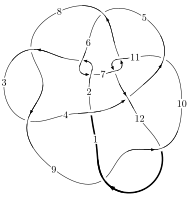
\includegraphics[width=112pt]{../../../GIT/diagram.site/Diagrams/png/1733_12a_0932.png}\\
\ \ \ A knot diagram\footnotemark}&
\allowdisplaybreaks
\textbf{Linearized knot diagam} \\
\cline{2-2}
 &
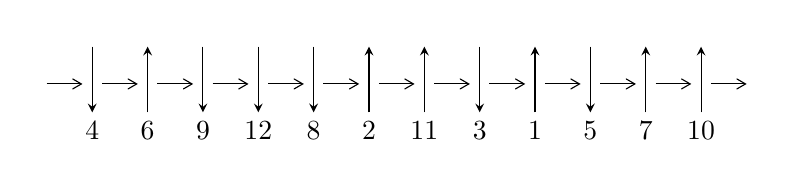
\begin{tikzpicture}[x=20pt, y=17pt]
	% nodes
	\node (C0) at (0, 0) {};
	\node (C1) at (1, 0) {};
	\node (C1U) at (1, +1) {};
	\node (C1D) at (1, -1) {4};

	\node (C2) at (2, 0) {};
	\node (C2U) at (2, +1) {};
	\node (C2D) at (2, -1) {6};

	\node (C3) at (3, 0) {};
	\node (C3U) at (3, +1) {};
	\node (C3D) at (3, -1) {9};

	\node (C4) at (4, 0) {};
	\node (C4U) at (4, +1) {};
	\node (C4D) at (4, -1) {12};

	\node (C5) at (5, 0) {};
	\node (C5U) at (5, +1) {};
	\node (C5D) at (5, -1) {8};

	\node (C6) at (6, 0) {};
	\node (C6U) at (6, +1) {};
	\node (C6D) at (6, -1) {2};

	\node (C7) at (7, 0) {};
	\node (C7U) at (7, +1) {};
	\node (C7D) at (7, -1) {11};

	\node (C8) at (8, 0) {};
	\node (C8U) at (8, +1) {};
	\node (C8D) at (8, -1) {3};

	\node (C9) at (9, 0) {};
	\node (C9U) at (9, +1) {};
	\node (C9D) at (9, -1) {1};

	\node (C10) at (10, 0) {};
	\node (C10U) at (10, +1) {};
	\node (C10D) at (10, -1) {5};

	\node (C11) at (11, 0) {};
	\node (C11U) at (11, +1) {};
	\node (C11D) at (11, -1) {7};

	\node (C12) at (12, 0) {};
	\node (C12U) at (12, +1) {};
	\node (C12D) at (12, -1) {10};
	\node (C13) at (13, 0) {};

	% arrows
	\draw[->,>={angle 60}]
	(C0) edge (C1) (C1) edge (C2) (C2) edge (C3) (C3) edge (C4) (C4) edge (C5) (C5) edge (C6) (C6) edge (C7) (C7) edge (C8) (C8) edge (C9) (C9) edge (C10) (C10) edge (C11) (C11) edge (C12) (C12) edge (C13) ;	\draw[->,>=stealth]
	(C1U) edge (C1D) (C2D) edge (C2U) (C3U) edge (C3D) (C4U) edge (C4D) (C5U) edge (C5D) (C6D) edge (C6U) (C7D) edge (C7U) (C8U) edge (C8D) (C9D) edge (C9U) (C10U) edge (C10D) (C11D) edge (C11U) (C12D) edge (C12U) ;
	\end{tikzpicture} \\
\hhline{~~} \\& 
\textbf{Solving Sequence} \\ \cline{2-2} 
 &
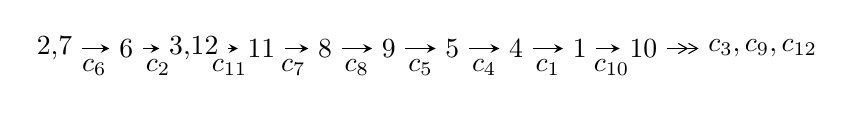
\begin{tikzpicture}[x=23pt, y=7pt]
	% node
	\node (A0) at (-1/8, 0) {2,7};
	\node (A1) at (1, 0) {6};
	\node (A2) at (33/16, 0) {3,12};
	\node (A3) at (25/8, 0) {11};
	\node (A4) at (33/8, 0) {8};
	\node (A5) at (41/8, 0) {9};
	\node (A6) at (49/8, 0) {5};
	\node (A7) at (57/8, 0) {4};
	\node (A8) at (65/8, 0) {1};
	\node (A9) at (73/8, 0) {10};
	\node (C1) at (1/2, -1) {$c_{6}$};
	\node (C2) at (3/2, -1) {$c_{2}$};
	\node (C3) at (21/8, -1) {$c_{11}$};
	\node (C4) at (29/8, -1) {$c_{7}$};
	\node (C5) at (37/8, -1) {$c_{8}$};
	\node (C6) at (45/8, -1) {$c_{5}$};
	\node (C7) at (53/8, -1) {$c_{4}$};
	\node (C8) at (61/8, -1) {$c_{1}$};
	\node (C9) at (69/8, -1) {$c_{10}$};
	\node (A10) at (11, 0) {$c_{3},c_{9},c_{12}$};

	% edge
	\draw[->,>=stealth]	
	(A0) edge (A1) (A1) edge (A2) (A2) edge (A3) (A3) edge (A4) (A4) edge (A5) (A5) edge (A6) (A6) edge (A7) (A7) edge (A8) (A8) edge (A9) ;
	\draw[->>,>={angle 60}]	
	(A9) edge (A10);
\end{tikzpicture} \\ 

\end{tabular} \\

\footnotetext{
The image of knot diagram is generated by the software ``\textbf{Draw programme}" developed by Andrew Bartholomew(\url{http://www.layer8.co.uk/maths/draw/index.htm\#Running-draw}), where we modified some parts for our purpose(\url{https://github.com/CATsTAILs/LinksPainter}).
}\phantom \\ \newline 
\centering \textbf{Ideals for irreducible components\footnotemark of $X_{\text{par}}$} 
 
\begin{align*}
I^u_{1}&=\langle 
-2.41105\times10^{799} u^{150}+6.29072\times10^{798} u^{149}+\cdots+1.72778\times10^{801} b+1.45209\times10^{805},\\
\phantom{I^u_{1}}&\phantom{= \langle  }-1.56739\times10^{805} u^{150}+3.30443\times10^{804} u^{149}+\cdots+1.09830\times10^{807} a+1.08834\times10^{811},\\
\phantom{I^u_{1}}&\phantom{= \langle  }u^{151}+50 u^{149}+\cdots-12000095 u-635671\rangle \\
I^u_{2}&=\langle 
-8.46792\times10^{33} u^{45}-3.69547\times10^{34} u^{44}+\cdots+1.19695\times10^{33} b+4.21370\times10^{34},\\
\phantom{I^u_{2}}&\phantom{= \langle  }5.75996\times10^{34} u^{45}+1.92741\times10^{35} u^{44}+\cdots+1.19695\times10^{33} a+1.44621\times10^{34},\;u^{46}+3 u^{45}+\cdots+6 u-1\rangle \\
\\
\end{align*}
\raggedright * 2 irreducible components of $\dim_{\mathbb{C}}=0$, with total 197 representations.\\
\footnotetext{All coefficients of polynomials are rational numbers. But the coefficients are sometimes approximated in decimal forms when there is not enough margin.}
\newpage
\renewcommand{\arraystretch}{1}
\centering \section*{I. $I^u_{1}= \langle -2.41\times10^{799} u^{150}+6.29\times10^{798} u^{149}+\cdots+1.73\times10^{801} b+1.45\times10^{805},\;-1.57\times10^{805} u^{150}+3.30\times10^{804} u^{149}+\cdots+1.10\times10^{807} a+1.09\times10^{811},\;u^{151}+50 u^{149}+\cdots-12000095 u-635671 \rangle$}
\flushleft \textbf{(i) Arc colorings}\\
\begin{tabular}{m{7pt} m{180pt} m{7pt} m{180pt} }
\flushright $a_{2}=$&$\begin{pmatrix}0\\u\end{pmatrix}$ \\
\flushright $a_{7}=$&$\begin{pmatrix}1\\0\end{pmatrix}$ \\
\flushright $a_{6}=$&$\begin{pmatrix}1\\u^2\end{pmatrix}$ \\
\flushright $a_{3}=$&$\begin{pmatrix}u\\u^3+u\end{pmatrix}$ \\
\flushright $a_{12}=$&$\begin{pmatrix}0.0142711 u^{150}-0.00300868 u^{149}+\cdots-180539. u-9909.32\\0.0139546 u^{150}-0.00364092 u^{149}+\cdots-147724. u-8404.37\end{pmatrix}$ \\
\flushright $a_{11}=$&$\begin{pmatrix}0.000316499 u^{150}+0.000632245 u^{149}+\cdots-32814.9 u-1504.94\\0.0139546 u^{150}-0.00364092 u^{149}+\cdots-147724. u-8404.37\end{pmatrix}$ \\
\flushright $a_{8}=$&$\begin{pmatrix}-0.0165871 u^{150}-0.0245620 u^{149}+\cdots+237804. u+12996.9\\0.0277901 u^{150}+0.00382596 u^{149}+\cdots-227726. u-11674.0\end{pmatrix}$ \\
\flushright $a_{9}=$&$\begin{pmatrix}-0.000639872 u^{150}-0.0193413 u^{149}+\cdots+135615. u+7941.56\\0.0243744 u^{150}+0.00465333 u^{149}+\cdots-257128. u-13410.6\end{pmatrix}$ \\
\flushright $a_{5}=$&$\begin{pmatrix}0.0114673 u^{150}-0.00964512 u^{149}+\cdots+91654.0 u+5521.75\\-0.00414055 u^{150}+0.0220643 u^{149}+\cdots-100097. u-5373.04\end{pmatrix}$ \\
\flushright $a_{4}=$&$\begin{pmatrix}0.00508007 u^{150}+0.00565611 u^{149}+\cdots-258979. u-15129.5\\0.00557188 u^{150}+0.0152743 u^{149}+\cdots-21634.5 u-1380.27\end{pmatrix}$ \\
\flushright $a_{1}=$&$\begin{pmatrix}-0.00519421 u^{150}-0.00101640 u^{149}+\cdots+157848. u+9370.88\\0.0297297 u^{150}-0.0138827 u^{149}+\cdots-29277.1 u-857.438\end{pmatrix}$ \\
\flushright $a_{10}=$&$\begin{pmatrix}-0.0264609 u^{150}-0.0231937 u^{149}+\cdots+416401. u+21980.2\\-0.00507039 u^{150}+0.00103144 u^{149}+\cdots+2108.46 u-139.846\end{pmatrix}$\\&\end{tabular}
\flushleft \textbf{(ii) Obstruction class $= -1$}\\~\\
\flushleft \textbf{(iii) Cusp Shapes $= -0.0706799 u^{150}+0.0664166 u^{149}+\cdots-832660. u-50135.3$}\\~\\
\newpage\renewcommand{\arraystretch}{1}
\flushleft \textbf{(iv) u-Polynomials at the component}\newline \\
\begin{tabular}{m{50pt}|m{274pt}}
Crossings & \hspace{64pt}u-Polynomials at each crossing \\
\hline $$\begin{aligned}c_{1}\end{aligned}$$&$\begin{aligned}
&u^{151}-15 u^{150}+\cdots-22057694910 u+1658964361
\end{aligned}$\\
\hline $$\begin{aligned}c_{2},c_{6}\end{aligned}$$&$\begin{aligned}
&u^{151}+50 u^{149}+\cdots-12000095 u-635671
\end{aligned}$\\
\hline $$\begin{aligned}c_{3},c_{8}\end{aligned}$$&$\begin{aligned}
&u^{151}- u^{150}+\cdots+40642 u+9299
\end{aligned}$\\
\hline $$\begin{aligned}c_{4}\end{aligned}$$&$\begin{aligned}
&u^{151}+3 u^{150}+\cdots+191957 u-6301
\end{aligned}$\\
\hline $$\begin{aligned}c_{5}\end{aligned}$$&$\begin{aligned}
&u^{151}-7 u^{150}+\cdots+13056495585 u-1546221241
\end{aligned}$\\
\hline $$\begin{aligned}c_{7},c_{11}\end{aligned}$$&$\begin{aligned}
&u^{151}-3 u^{150}+\cdots-44403 u-18287
\end{aligned}$\\
\hline $$\begin{aligned}c_{9},c_{12}\end{aligned}$$&$\begin{aligned}
&u^{151}+5 u^{150}+\cdots+31 u+1
\end{aligned}$\\
\hline $$\begin{aligned}c_{10}\end{aligned}$$&$\begin{aligned}
&u^{151}- u^{150}+\cdots+2070354906 u-331170187
\end{aligned}$\\
\hline
\end{tabular}\\~\\
\newpage\renewcommand{\arraystretch}{1}
\flushleft \textbf{(v) Riley Polynomials at the component}\newline \\
\begin{tabular}{m{50pt}|m{274pt}}
Crossings & \hspace{64pt}Riley Polynomials at each crossing \\
\hline $$\begin{aligned}c_{1}\end{aligned}$$&$\begin{aligned}
&y^{151}-69 y^{150}+\cdots+1.51\times10^{20} y-2.75\times10^{18}
\end{aligned}$\\
\hline $$\begin{aligned}c_{2},c_{6}\end{aligned}$$&$\begin{aligned}
&y^{151}+100 y^{150}+\cdots-2921995709471 y-404077620241
\end{aligned}$\\
\hline $$\begin{aligned}c_{3},c_{8}\end{aligned}$$&$\begin{aligned}
&y^{151}-139 y^{150}+\cdots-4712909788 y-86471401
\end{aligned}$\\
\hline $$\begin{aligned}c_{4}\end{aligned}$$&$\begin{aligned}
&y^{151}-17 y^{150}+\cdots+25879162721 y-39702601
\end{aligned}$\\
\hline $$\begin{aligned}c_{5}\end{aligned}$$&$\begin{aligned}
&y^{151}-83 y^{150}+\cdots+1.37\times10^{19} y-2.39\times10^{18}
\end{aligned}$\\
\hline $$\begin{aligned}c_{7},c_{11}\end{aligned}$$&$\begin{aligned}
&y^{151}+93 y^{150}+\cdots-13900794685 y-334414369
\end{aligned}$\\
\hline $$\begin{aligned}c_{9},c_{12}\end{aligned}$$&$\begin{aligned}
&y^{151}+117 y^{150}+\cdots-69 y-1
\end{aligned}$\\
\hline $$\begin{aligned}c_{10}\end{aligned}$$&$\begin{aligned}
&y^{151}-61 y^{150}+\cdots+8.43\times10^{18} y-1.10\times10^{17}
\end{aligned}$\\
\hline
\end{tabular}\\~\\
\newpage\flushleft \textbf{(vi) Complex Volumes and Cusp Shapes}
$$\begin{array}{c|c|c}  
\text{Solutions to }I^u_{1}& \I (\text{vol} + \sqrt{-1}CS) & \text{Cusp shape}\\
 \hline 
\begin{aligned}
u &= \phantom{-}0.865429 + 0.496053 I \\
a &= -0.268547 - 0.144131 I \\
b &= -0.169743 + 0.653881 I\end{aligned}
 & \phantom{-}0.24032 + 1.74389 I & \phantom{-0.000000 } 0 \\ \hline\begin{aligned}
u &= \phantom{-}0.865429 - 0.496053 I \\
a &= -0.268547 + 0.144131 I \\
b &= -0.169743 - 0.653881 I\end{aligned}
 & \phantom{-}0.24032 - 1.74389 I & \phantom{-0.000000 } 0 \\ \hline\begin{aligned}
u &= \phantom{-}0.544660 + 0.865037 I \\
a &= \phantom{-}1.98651 + 1.02388 I \\
b &= \phantom{-}0.263339 + 1.062250 I\end{aligned}
 & -5.22891 + 4.97394 I & \phantom{-0.000000 } 0 \\ \hline\begin{aligned}
u &= \phantom{-}0.544660 - 0.865037 I \\
a &= \phantom{-}1.98651 - 1.02388 I \\
b &= \phantom{-}0.263339 - 1.062250 I\end{aligned}
 & -5.22891 - 4.97394 I & \phantom{-0.000000 } 0 \\ \hline\begin{aligned}
u &= -1.02743\phantom{ +0.000000I} \\
a &= \phantom{-}2.97107\phantom{ +0.000000I} \\
b &= \phantom{-}1.32448\phantom{ +0.000000I}\end{aligned}
 & \phantom{-}3.05308\phantom{ +0.000000I} & \phantom{-0.000000 } 0 \\ \hline\begin{aligned}
u &= -0.242033 + 1.033150 I \\
a &= -1.73031 + 1.26498 I \\
b &= -0.447359 + 0.918474 I\end{aligned}
 & -7.80679 - 9.01651 I & \phantom{-0.000000 } 0 \\ \hline\begin{aligned}
u &= -0.242033 - 1.033150 I \\
a &= -1.73031 - 1.26498 I \\
b &= -0.447359 - 0.918474 I\end{aligned}
 & -7.80679 + 9.01651 I & \phantom{-0.000000 } 0 \\ \hline\begin{aligned}
u &= \phantom{-}0.530409 + 0.774022 I \\
a &= -0.995330 + 0.824807 I \\
b &= -0.325630 + 0.719551 I\end{aligned}
 & -0.139921 + 0.875960 I & \phantom{-0.000000 } 0 \\ \hline\begin{aligned}
u &= \phantom{-}0.530409 - 0.774022 I \\
a &= -0.995330 - 0.824807 I \\
b &= -0.325630 - 0.719551 I\end{aligned}
 & -0.139921 - 0.875960 I & \phantom{-0.000000 } 0 \\ \hline\begin{aligned}
u &= \phantom{-}0.243570 + 1.042540 I \\
a &= -1.15722 + 1.81109 I \\
b &= -0.078889 - 0.972468 I\end{aligned}
 & -0.83258 + 2.48333 I & \phantom{-0.000000 } 0\\
 \hline 
 \end{array}$$\newpage$$\begin{array}{c|c|c}  
\text{Solutions to }I^u_{1}& \I (\text{vol} + \sqrt{-1}CS) & \text{Cusp shape}\\
 \hline 
\begin{aligned}
u &= \phantom{-}0.243570 - 1.042540 I \\
a &= -1.15722 - 1.81109 I \\
b &= -0.078889 + 0.972468 I\end{aligned}
 & -0.83258 - 2.48333 I & \phantom{-0.000000 } 0 \\ \hline\begin{aligned}
u &= \phantom{-}1.061410 + 0.143447 I \\
a &= \phantom{-}1.90202 + 0.28675 I \\
b &= \phantom{-}0.947695 + 0.058209 I\end{aligned}
 & -5.81650 + 7.46022 I & \phantom{-0.000000 } 0 \\ \hline\begin{aligned}
u &= \phantom{-}1.061410 - 0.143447 I \\
a &= \phantom{-}1.90202 - 0.28675 I \\
b &= \phantom{-}0.947695 - 0.058209 I\end{aligned}
 & -5.81650 - 7.46022 I & \phantom{-0.000000 } 0 \\ \hline\begin{aligned}
u &= \phantom{-}0.129607 + 1.069170 I \\
a &= \phantom{-}0.05263 - 2.20256 I \\
b &= -0.042773 + 1.024220 I\end{aligned}
 & -4.47865 - 1.10856 I & \phantom{-0.000000 } 0 \\ \hline\begin{aligned}
u &= \phantom{-}0.129607 - 1.069170 I \\
a &= \phantom{-}0.05263 + 2.20256 I \\
b &= -0.042773 - 1.024220 I\end{aligned}
 & -4.47865 + 1.10856 I & \phantom{-0.000000 } 0 \\ \hline\begin{aligned}
u &= -0.265402 + 1.052710 I \\
a &= \phantom{-}1.54598 - 0.57846 I \\
b &= \phantom{-}0.522807 - 0.919801 I\end{aligned}
 & -3.35425 - 5.50168 I & \phantom{-0.000000 } 0 \\ \hline\begin{aligned}
u &= -0.265402 - 1.052710 I \\
a &= \phantom{-}1.54598 + 0.57846 I \\
b &= \phantom{-}0.522807 + 0.919801 I\end{aligned}
 & -3.35425 + 5.50168 I & \phantom{-0.000000 } 0 \\ \hline\begin{aligned}
u &= -0.900947 + 0.097057 I \\
a &= \phantom{-}0.337167 - 0.367659 I \\
b &= \phantom{-}0.214532 - 1.215350 I\end{aligned}
 & -10.20030 - 3.80821 I & \phantom{-0.000000 } 0 \\ \hline\begin{aligned}
u &= -0.900947 - 0.097057 I \\
a &= \phantom{-}0.337167 + 0.367659 I \\
b &= \phantom{-}0.214532 + 1.215350 I\end{aligned}
 & -10.20030 + 3.80821 I & \phantom{-0.000000 } 0 \\ \hline\begin{aligned}
u &= -0.298443 + 0.844307 I \\
a &= -0.951262 - 0.856924 I \\
b &= \phantom{-}0.311635 - 0.762574 I\end{aligned}
 & -10.66430 - 2.51485 I & \phantom{-0.000000 } 0\\
 \hline 
 \end{array}$$\newpage$$\begin{array}{c|c|c}  
\text{Solutions to }I^u_{1}& \I (\text{vol} + \sqrt{-1}CS) & \text{Cusp shape}\\
 \hline 
\begin{aligned}
u &= -0.298443 - 0.844307 I \\
a &= -0.951262 + 0.856924 I \\
b &= \phantom{-}0.311635 + 0.762574 I\end{aligned}
 & -10.66430 + 2.51485 I & \phantom{-0.000000 } 0 \\ \hline\begin{aligned}
u &= \phantom{-}0.638574 + 0.902465 I \\
a &= -1.64056 - 0.23236 I \\
b &= -0.290932 - 0.945919 I\end{aligned}
 & -0.86401 + 3.67685 I & \phantom{-0.000000 } 0 \\ \hline\begin{aligned}
u &= \phantom{-}0.638574 - 0.902465 I \\
a &= -1.64056 + 0.23236 I \\
b &= -0.290932 + 0.945919 I\end{aligned}
 & -0.86401 - 3.67685 I & \phantom{-0.000000 } 0 \\ \hline\begin{aligned}
u &= \phantom{-}0.430723 + 1.021410 I \\
a &= \phantom{-}0.367353 - 0.044669 I \\
b &= \phantom{-}0.587542 - 0.252811 I\end{aligned}
 & -2.11097 + 2.48449 I & \phantom{-0.000000 } 0 \\ \hline\begin{aligned}
u &= \phantom{-}0.430723 - 1.021410 I \\
a &= \phantom{-}0.367353 + 0.044669 I \\
b &= \phantom{-}0.587542 + 0.252811 I\end{aligned}
 & -2.11097 - 2.48449 I & \phantom{-0.000000 } 0 \\ \hline\begin{aligned}
u &= \phantom{-}0.224900 + 0.861854 I \\
a &= \phantom{-}1.98744 - 0.65991 I \\
b &= \phantom{-}0.268852 - 0.617564 I\end{aligned}
 & -3.78934 + 2.50891 I & \phantom{-0.000000 } 0 \\ \hline\begin{aligned}
u &= \phantom{-}0.224900 - 0.861854 I \\
a &= \phantom{-}1.98744 + 0.65991 I \\
b &= \phantom{-}0.268852 + 0.617564 I\end{aligned}
 & -3.78934 - 2.50891 I & \phantom{-0.000000 } 0 \\ \hline\begin{aligned}
u &= -0.309284 + 1.075300 I \\
a &= \phantom{-}0.725149 + 0.242007 I \\
b &= \phantom{-}1.039710 - 0.692197 I\end{aligned}
 & -8.23597 - 4.81426 I & \phantom{-0.000000 } 0 \\ \hline\begin{aligned}
u &= -0.309284 - 1.075300 I \\
a &= \phantom{-}0.725149 - 0.242007 I \\
b &= \phantom{-}1.039710 + 0.692197 I\end{aligned}
 & -8.23597 + 4.81426 I & \phantom{-0.000000 } 0 \\ \hline\begin{aligned}
u &= -0.872510 + 0.109907 I \\
a &= -0.341550 - 0.900308 I \\
b &= -0.376088 - 0.847274 I\end{aligned}
 & -3.69772 - 1.50417 I & \phantom{-0.000000 } 0\\
 \hline 
 \end{array}$$\newpage$$\begin{array}{c|c|c}  
\text{Solutions to }I^u_{1}& \I (\text{vol} + \sqrt{-1}CS) & \text{Cusp shape}\\
 \hline 
\begin{aligned}
u &= -0.872510 - 0.109907 I \\
a &= -0.341550 + 0.900308 I \\
b &= -0.376088 + 0.847274 I\end{aligned}
 & -3.69772 + 1.50417 I & \phantom{-0.000000 } 0 \\ \hline\begin{aligned}
u &= -0.277223 + 1.095000 I \\
a &= -1.266940 - 0.089463 I \\
b &= -0.657102 + 0.996844 I\end{aligned}
 & -6.51741 - 2.25945 I & \phantom{-0.000000 } 0 \\ \hline\begin{aligned}
u &= -0.277223 - 1.095000 I \\
a &= -1.266940 + 0.089463 I \\
b &= -0.657102 - 0.996844 I\end{aligned}
 & -6.51741 + 2.25945 I & \phantom{-0.000000 } 0 \\ \hline\begin{aligned}
u &= -0.464801 + 0.730573 I \\
a &= \phantom{-}1.82903 - 1.34189 I \\
b &= -0.130016 - 1.106320 I\end{aligned}
 & -7.01390 + 6.25687 I & \phantom{-0.000000 } 0 \\ \hline\begin{aligned}
u &= -0.464801 - 0.730573 I \\
a &= \phantom{-}1.82903 + 1.34189 I \\
b &= -0.130016 + 1.106320 I\end{aligned}
 & -7.01390 - 6.25687 I & \phantom{-0.000000 } 0 \\ \hline\begin{aligned}
u &= -0.223093 + 1.116750 I \\
a &= -0.554263 - 0.411086 I \\
b &= -1.328580 - 0.018051 I\end{aligned}
 & -3.61376 - 6.53097 I & \phantom{-0.000000 } 0 \\ \hline\begin{aligned}
u &= -0.223093 - 1.116750 I \\
a &= -0.554263 + 0.411086 I \\
b &= -1.328580 + 0.018051 I\end{aligned}
 & -3.61376 + 6.53097 I & \phantom{-0.000000 } 0 \\ \hline\begin{aligned}
u &= -0.157681 + 1.132260 I \\
a &= -0.442803 - 0.705338 I \\
b &= -0.833943 - 0.288319 I\end{aligned}
 & -5.15589 + 2.04118 I & \phantom{-0.000000 } 0 \\ \hline\begin{aligned}
u &= -0.157681 - 1.132260 I \\
a &= -0.442803 + 0.705338 I \\
b &= -0.833943 + 0.288319 I\end{aligned}
 & -5.15589 - 2.04118 I & \phantom{-0.000000 } 0 \\ \hline\begin{aligned}
u &= -0.342353 + 1.110630 I \\
a &= -0.414558 - 0.051773 I \\
b &= -0.685358 + 0.403556 I\end{aligned}
 & -5.33499 - 3.86310 I & \phantom{-0.000000 } 0\\
 \hline 
 \end{array}$$\newpage$$\begin{array}{c|c|c}  
\text{Solutions to }I^u_{1}& \I (\text{vol} + \sqrt{-1}CS) & \text{Cusp shape}\\
 \hline 
\begin{aligned}
u &= -0.342353 - 1.110630 I \\
a &= -0.414558 + 0.051773 I \\
b &= -0.685358 - 0.403556 I\end{aligned}
 & -5.33499 + 3.86310 I & \phantom{-0.000000 } 0 \\ \hline\begin{aligned}
u &= -0.220364 + 1.142150 I \\
a &= \phantom{-}0.586780 + 0.498797 I \\
b &= \phantom{-}1.211050 + 0.255080 I\end{aligned}
 & -0.25364 - 1.94629 I & \phantom{-0.000000 } 0 \\ \hline\begin{aligned}
u &= -0.220364 - 1.142150 I \\
a &= \phantom{-}0.586780 - 0.498797 I \\
b &= \phantom{-}1.211050 - 0.255080 I\end{aligned}
 & -0.25364 + 1.94629 I & \phantom{-0.000000 } 0 \\ \hline\begin{aligned}
u &= \phantom{-}0.011102 + 1.168060 I \\
a &= -1.81662 - 0.57133 I \\
b &= -0.590866 - 0.686481 I\end{aligned}
 & -7.14480 - 4.85538 I & \phantom{-0.000000 } 0 \\ \hline\begin{aligned}
u &= \phantom{-}0.011102 - 1.168060 I \\
a &= -1.81662 + 0.57133 I \\
b &= -0.590866 + 0.686481 I\end{aligned}
 & -7.14480 + 4.85538 I & \phantom{-0.000000 } 0 \\ \hline\begin{aligned}
u &= \phantom{-}0.023141 + 1.180660 I \\
a &= \phantom{-}0.589991 - 0.360111 I \\
b &= \phantom{-}0.81303 + 1.59511 I\end{aligned}
 & -10.60990 + 3.42667 I & \phantom{-0.000000 } 0 \\ \hline\begin{aligned}
u &= \phantom{-}0.023141 - 1.180660 I \\
a &= \phantom{-}0.589991 + 0.360111 I \\
b &= \phantom{-}0.81303 - 1.59511 I\end{aligned}
 & -10.60990 - 3.42667 I & \phantom{-0.000000 } 0 \\ \hline\begin{aligned}
u &= \phantom{-}0.022790 + 1.186940 I \\
a &= \phantom{-}1.287750 + 0.451193 I \\
b &= \phantom{-}0.748027 + 0.595783 I\end{aligned}
 & -2.38157 - 0.70111 I & \phantom{-0.000000 } 0 \\ \hline\begin{aligned}
u &= \phantom{-}0.022790 - 1.186940 I \\
a &= \phantom{-}1.287750 - 0.451193 I \\
b &= \phantom{-}0.748027 - 0.595783 I\end{aligned}
 & -2.38157 + 0.70111 I & \phantom{-0.000000 } 0 \\ \hline\begin{aligned}
u &= \phantom{-}0.517442 + 0.619554 I \\
a &= -0.16912 - 1.85951 I \\
b &= -0.026688 - 1.051580 I\end{aligned}
 & -4.59461 - 0.62986 I & \phantom{-0.000000 } 0\\
 \hline 
 \end{array}$$\newpage$$\begin{array}{c|c|c}  
\text{Solutions to }I^u_{1}& \I (\text{vol} + \sqrt{-1}CS) & \text{Cusp shape}\\
 \hline 
\begin{aligned}
u &= \phantom{-}0.517442 - 0.619554 I \\
a &= -0.16912 + 1.85951 I \\
b &= -0.026688 + 1.051580 I\end{aligned}
 & -4.59461 + 0.62986 I & \phantom{-0.000000 } 0 \\ \hline\begin{aligned}
u &= \phantom{-}0.236059 + 0.770587 I \\
a &= \phantom{-}3.37427 - 1.48040 I \\
b &= \phantom{-}0.053774 + 0.746655 I\end{aligned}
 & -5.31765 + 5.61402 I & \phantom{-0.000000 } 0 \\ \hline\begin{aligned}
u &= \phantom{-}0.236059 - 0.770587 I \\
a &= \phantom{-}3.37427 + 1.48040 I \\
b &= \phantom{-}0.053774 - 0.746655 I\end{aligned}
 & -5.31765 - 5.61402 I & \phantom{-0.000000 } 0 \\ \hline\begin{aligned}
u &= -0.049615 + 1.202690 I \\
a &= \phantom{-}1.05417 - 1.15879 I \\
b &= \phantom{-}0.525700 + 1.129350 I\end{aligned}
 & -12.49350 + 1.20983 I & \phantom{-0.000000 } 0 \\ \hline\begin{aligned}
u &= -0.049615 - 1.202690 I \\
a &= \phantom{-}1.05417 + 1.15879 I \\
b &= \phantom{-}0.525700 - 1.129350 I\end{aligned}
 & -12.49350 - 1.20983 I & \phantom{-0.000000 } 0 \\ \hline\begin{aligned}
u &= \phantom{-}0.584037 + 0.541159 I \\
a &= \phantom{-}0.207858 + 0.476487 I \\
b &= \phantom{-}0.126923 + 0.752522 I\end{aligned}
 & -0.147746 + 1.239980 I & \phantom{-0.000000 } 0 \\ \hline\begin{aligned}
u &= \phantom{-}0.584037 - 0.541159 I \\
a &= \phantom{-}0.207858 - 0.476487 I \\
b &= \phantom{-}0.126923 - 0.752522 I\end{aligned}
 & -0.147746 - 1.239980 I & \phantom{-0.000000 } 0 \\ \hline\begin{aligned}
u &= \phantom{-}0.422029 + 0.674736 I \\
a &= -0.208595 + 0.256715 I \\
b &= -0.019292 + 0.489149 I\end{aligned}
 & -0.150324 + 1.191570 I & \phantom{-0.000000 } 0 \\ \hline\begin{aligned}
u &= \phantom{-}0.422029 - 0.674736 I \\
a &= -0.208595 - 0.256715 I \\
b &= -0.019292 - 0.489149 I\end{aligned}
 & -0.150324 - 1.191570 I & \phantom{-0.000000 } 0 \\ \hline\begin{aligned}
u &= -0.005809 + 1.209250 I \\
a &= -0.775376 + 0.595738 I \\
b &= -0.67186 - 1.30048 I\end{aligned}
 & -7.68026 + 2.12334 I & \phantom{-0.000000 } 0\\
 \hline 
 \end{array}$$\newpage$$\begin{array}{c|c|c}  
\text{Solutions to }I^u_{1}& \I (\text{vol} + \sqrt{-1}CS) & \text{Cusp shape}\\
 \hline 
\begin{aligned}
u &= -0.005809 - 1.209250 I \\
a &= -0.775376 - 0.595738 I \\
b &= -0.67186 + 1.30048 I\end{aligned}
 & -7.68026 - 2.12334 I & \phantom{-0.000000 } 0 \\ \hline\begin{aligned}
u &= -0.780610 + 0.123255 I \\
a &= -0.705884 - 0.912679 I \\
b &= -0.490970 - 1.233500 I\end{aligned}
 & -4.51635 + 8.61713 I & \phantom{-0.000000 } 0 \\ \hline\begin{aligned}
u &= -0.780610 - 0.123255 I \\
a &= -0.705884 + 0.912679 I \\
b &= -0.490970 + 1.233500 I\end{aligned}
 & -4.51635 - 8.61713 I & \phantom{-0.000000 } 0 \\ \hline\begin{aligned}
u &= \phantom{-}0.889337 + 0.826648 I \\
a &= -0.921696 - 0.254962 I \\
b &= -0.261736 - 0.935220 I\end{aligned}
 & -0.68326 + 4.13158 I & \phantom{-0.000000 } 0 \\ \hline\begin{aligned}
u &= \phantom{-}0.889337 - 0.826648 I \\
a &= -0.921696 + 0.254962 I \\
b &= -0.261736 + 0.935220 I\end{aligned}
 & -0.68326 - 4.13158 I & \phantom{-0.000000 } 0 \\ \hline\begin{aligned}
u &= -0.551982 + 0.557205 I \\
a &= -1.09061 + 1.48623 I \\
b &= \phantom{-}0.114194 + 1.055160 I\end{aligned}
 & -1.98667 + 2.38452 I & \phantom{-0.000000 } 0 \\ \hline\begin{aligned}
u &= -0.551982 - 0.557205 I \\
a &= -1.09061 - 1.48623 I \\
b &= \phantom{-}0.114194 - 1.055160 I\end{aligned}
 & -1.98667 - 2.38452 I & \phantom{-0.000000 } 0 \\ \hline\begin{aligned}
u &= -0.536840 + 1.099030 I \\
a &= -0.0499611 + 0.0855238 I \\
b &= -0.153416 + 0.527398 I\end{aligned}
 & -5.18855 - 3.89854 I & \phantom{-0.000000 } 0 \\ \hline\begin{aligned}
u &= -0.536840 - 1.099030 I \\
a &= -0.0499611 - 0.0855238 I \\
b &= -0.153416 - 0.527398 I\end{aligned}
 & -5.18855 + 3.89854 I & \phantom{-0.000000 } 0 \\ \hline\begin{aligned}
u &= -0.026662 + 1.226840 I \\
a &= -1.031000 - 0.148899 I \\
b &= -1.104570 - 0.731839 I\end{aligned}
 & -5.21433 + 4.11104 I & \phantom{-0.000000 } 0\\
 \hline 
 \end{array}$$\newpage$$\begin{array}{c|c|c}  
\text{Solutions to }I^u_{1}& \I (\text{vol} + \sqrt{-1}CS) & \text{Cusp shape}\\
 \hline 
\begin{aligned}
u &= -0.026662 - 1.226840 I \\
a &= -1.031000 + 0.148899 I \\
b &= -1.104570 + 0.731839 I\end{aligned}
 & -5.21433 - 4.11104 I & \phantom{-0.000000 } 0 \\ \hline\begin{aligned}
u &= -0.740949 + 0.210292 I \\
a &= \phantom{-}0.779348 + 1.100260 I \\
b &= \phantom{-}0.497411 + 1.187600 I\end{aligned}
 & -0.53238 + 4.13880 I & \phantom{-0.000000 } 0 \\ \hline\begin{aligned}
u &= -0.740949 - 0.210292 I \\
a &= \phantom{-}0.779348 - 1.100260 I \\
b &= \phantom{-}0.497411 - 1.187600 I\end{aligned}
 & -0.53238 - 4.13880 I & \phantom{-0.000000 } 0 \\ \hline\begin{aligned}
u &= \phantom{-}0.088278 + 1.227140 I \\
a &= -0.313874 + 0.509264 I \\
b &= -0.29913 - 1.62071 I\end{aligned}
 & -9.64732 + 0.27043 I & \phantom{-0.000000 } 0 \\ \hline\begin{aligned}
u &= \phantom{-}0.088278 - 1.227140 I \\
a &= -0.313874 - 0.509264 I \\
b &= -0.29913 + 1.62071 I\end{aligned}
 & -9.64732 - 0.27043 I & \phantom{-0.000000 } 0 \\ \hline\begin{aligned}
u &= -0.718372 + 0.130287 I \\
a &= \phantom{-}0.757620 + 0.576115 I \\
b &= \phantom{-}0.705582 + 0.317866 I\end{aligned}
 & -5.57819 + 0.95362 I & \phantom{-0.000000 } 0 \\ \hline\begin{aligned}
u &= -0.718372 - 0.130287 I \\
a &= \phantom{-}0.757620 - 0.576115 I \\
b &= \phantom{-}0.705582 - 0.317866 I\end{aligned}
 & -5.57819 - 0.95362 I & \phantom{-0.000000 } 0 \\ \hline\begin{aligned}
u &= \phantom{-}0.694922 + 0.180838 I \\
a &= -1.76585 - 1.29723 I \\
b &= -0.393984 - 0.079643 I\end{aligned}
 & \phantom{-}0.93187 + 2.46526 I & \phantom{-0.000000 } 0 \\ \hline\begin{aligned}
u &= \phantom{-}0.694922 - 0.180838 I \\
a &= -1.76585 + 1.29723 I \\
b &= -0.393984 + 0.079643 I\end{aligned}
 & \phantom{-}0.93187 - 2.46526 I & \phantom{-0.000000 } 0 \\ \hline\begin{aligned}
u &= -0.338018 + 1.238260 I \\
a &= \phantom{-}0.097805 + 0.281128 I \\
b &= \phantom{-}0.653616 + 0.080122 I\end{aligned}
 & -9.70476 - 2.81066 I & \phantom{-0.000000 } 0\\
 \hline 
 \end{array}$$\newpage$$\begin{array}{c|c|c}  
\text{Solutions to }I^u_{1}& \I (\text{vol} + \sqrt{-1}CS) & \text{Cusp shape}\\
 \hline 
\begin{aligned}
u &= -0.338018 - 1.238260 I \\
a &= \phantom{-}0.097805 - 0.281128 I \\
b &= \phantom{-}0.653616 - 0.080122 I\end{aligned}
 & -9.70476 + 2.81066 I & \phantom{-0.000000 } 0 \\ \hline\begin{aligned}
u &= \phantom{-}0.684993 + 0.202292 I \\
a &= \phantom{-}0.573798 - 0.249534 I \\
b &= \phantom{-}0.337461 + 0.567327 I\end{aligned}
 & \phantom{-}0.03770 + 1.55930 I & \phantom{-0.000000 } 0 \\ \hline\begin{aligned}
u &= \phantom{-}0.684993 - 0.202292 I \\
a &= \phantom{-}0.573798 + 0.249534 I \\
b &= \phantom{-}0.337461 - 0.567327 I\end{aligned}
 & \phantom{-}0.03770 - 1.55930 I & \phantom{-0.000000 } 0 \\ \hline\begin{aligned}
u &= \phantom{-}0.075513 + 1.297180 I \\
a &= \phantom{-}0.352206 - 0.683539 I \\
b &= \phantom{-}0.319398 + 1.358910 I\end{aligned}
 & -6.12604 + 2.87334 I & \phantom{-0.000000 } 0 \\ \hline\begin{aligned}
u &= \phantom{-}0.075513 - 1.297180 I \\
a &= \phantom{-}0.352206 + 0.683539 I \\
b &= \phantom{-}0.319398 - 1.358910 I\end{aligned}
 & -6.12604 - 2.87334 I & \phantom{-0.000000 } 0 \\ \hline\begin{aligned}
u &= -0.383926 + 1.242470 I \\
a &= -1.58358 - 0.48738 I \\
b &= -0.622129 + 1.263270 I\end{aligned}
 & -7.94194 - 3.63600 I & \phantom{-0.000000 } 0 \\ \hline\begin{aligned}
u &= -0.383926 - 1.242470 I \\
a &= -1.58358 + 0.48738 I \\
b &= -0.622129 - 1.263270 I\end{aligned}
 & -7.94194 + 3.63600 I & \phantom{-0.000000 } 0 \\ \hline\begin{aligned}
u &= \phantom{-}0.402982 + 1.236750 I \\
a &= \phantom{-}0.945176 - 0.790667 I \\
b &= \phantom{-}0.278268 + 1.025640 I\end{aligned}
 & -4.26480 + 5.68885 I & \phantom{-0.000000 } 0 \\ \hline\begin{aligned}
u &= \phantom{-}0.402982 - 1.236750 I \\
a &= \phantom{-}0.945176 + 0.790667 I \\
b &= \phantom{-}0.278268 - 1.025640 I\end{aligned}
 & -4.26480 - 5.68885 I & \phantom{-0.000000 } 0 \\ \hline\begin{aligned}
u &= -0.697140\phantom{ +0.000000I} \\
a &= -0.683406\phantom{ +0.000000I} \\
b &= -0.509534\phantom{ +0.000000I}\end{aligned}
 & -2.09215\phantom{ +0.000000I} & \phantom{-0.000000 } 0\\
 \hline 
 \end{array}$$\newpage$$\begin{array}{c|c|c}  
\text{Solutions to }I^u_{1}& \I (\text{vol} + \sqrt{-1}CS) & \text{Cusp shape}\\
 \hline 
\begin{aligned}
u &= -1.126950 + 0.673716 I \\
a &= \phantom{-}0.566957 - 0.619186 I \\
b &= -0.016370 - 1.065140 I\end{aligned}
 & -3.58274 - 2.29086 I & \phantom{-0.000000 } 0 \\ \hline\begin{aligned}
u &= -1.126950 - 0.673716 I \\
a &= \phantom{-}0.566957 + 0.619186 I \\
b &= -0.016370 + 1.065140 I\end{aligned}
 & -3.58274 + 2.29086 I & \phantom{-0.000000 } 0 \\ \hline\begin{aligned}
u &= -0.397256 + 1.257510 I \\
a &= \phantom{-}1.37131 + 0.49851 I \\
b &= \phantom{-}0.60803 - 1.35519 I\end{aligned}
 & -3.94419 - 8.42195 I & \phantom{-0.000000 } 0 \\ \hline\begin{aligned}
u &= -0.397256 - 1.257510 I \\
a &= \phantom{-}1.37131 - 0.49851 I \\
b &= \phantom{-}0.60803 + 1.35519 I\end{aligned}
 & -3.94419 + 8.42195 I & \phantom{-0.000000 } 0 \\ \hline\begin{aligned}
u &= -0.413412 + 1.260990 I \\
a &= -1.307750 - 0.524959 I \\
b &= -0.58013 + 1.40879 I\end{aligned}
 & -8.0994 - 13.0437 I & \phantom{-0.000000 } 0 \\ \hline\begin{aligned}
u &= -0.413412 - 1.260990 I \\
a &= -1.307750 + 0.524959 I \\
b &= -0.58013 - 1.40879 I\end{aligned}
 & -8.0994 + 13.0437 I & \phantom{-0.000000 } 0 \\ \hline\begin{aligned}
u &= \phantom{-}1.336700 + 0.058716 I \\
a &= \phantom{-}0.944357 - 0.873808 I \\
b &= \phantom{-}0.486507 - 1.325130 I\end{aligned}
 & -10.0374 - 12.6004 I & \phantom{-0.000000 } 0 \\ \hline\begin{aligned}
u &= \phantom{-}1.336700 - 0.058716 I \\
a &= \phantom{-}0.944357 + 0.873808 I \\
b &= \phantom{-}0.486507 + 1.325130 I\end{aligned}
 & -10.0374 + 12.6004 I & \phantom{-0.000000 } 0 \\ \hline\begin{aligned}
u &= -0.603853 + 0.263884 I \\
a &= -0.802637 - 0.308458 I \\
b &= -0.405901 + 1.036810 I\end{aligned}
 & -4.74200 - 3.35284 I & \phantom{-0.000000 } 0 \\ \hline\begin{aligned}
u &= -0.603853 - 0.263884 I \\
a &= -0.802637 + 0.308458 I \\
b &= -0.405901 - 1.036810 I\end{aligned}
 & -4.74200 + 3.35284 I & \phantom{-0.000000 } 0\\
 \hline 
 \end{array}$$\newpage$$\begin{array}{c|c|c}  
\text{Solutions to }I^u_{1}& \I (\text{vol} + \sqrt{-1}CS) & \text{Cusp shape}\\
 \hline 
\begin{aligned}
u &= -0.020947 + 1.371670 I \\
a &= -0.233442 + 0.731342 I \\
b &= -0.376381 - 1.258700 I\end{aligned}
 & -9.67693 + 6.00190 I & \phantom{-0.000000 } 0 \\ \hline\begin{aligned}
u &= -0.020947 - 1.371670 I \\
a &= -0.233442 - 0.731342 I \\
b &= -0.376381 + 1.258700 I\end{aligned}
 & -9.67693 - 6.00190 I & \phantom{-0.000000 } 0 \\ \hline\begin{aligned}
u &= -0.504923 + 1.297790 I \\
a &= \phantom{-}0.0816543 - 0.0797088 I \\
b &= -0.273500 - 0.474278 I\end{aligned}
 & -7.97110 - 6.61693 I & \phantom{-0.000000 } 0 \\ \hline\begin{aligned}
u &= -0.504923 - 1.297790 I \\
a &= \phantom{-}0.0816543 + 0.0797088 I \\
b &= -0.273500 + 0.474278 I\end{aligned}
 & -7.97110 + 6.61693 I & \phantom{-0.000000 } 0 \\ \hline\begin{aligned}
u &= \phantom{-}1.283560 + 0.549496 I \\
a &= \phantom{-}1.07012 - 1.23907 I \\
b &= \phantom{-}0.61326 - 1.34358 I\end{aligned}
 & -9.38239 + 1.82696 I & \phantom{-0.000000 } 0 \\ \hline\begin{aligned}
u &= \phantom{-}1.283560 - 0.549496 I \\
a &= \phantom{-}1.07012 + 1.23907 I \\
b &= \phantom{-}0.61326 + 1.34358 I\end{aligned}
 & -9.38239 - 1.82696 I & \phantom{-0.000000 } 0 \\ \hline\begin{aligned}
u &= -0.464924 + 1.330000 I \\
a &= \phantom{-}1.136870 + 0.564568 I \\
b &= \phantom{-}0.314220 - 1.378770 I\end{aligned}
 & -14.5302 - 8.7392 I & \phantom{-0.000000 } 0 \\ \hline\begin{aligned}
u &= -0.464924 - 1.330000 I \\
a &= \phantom{-}1.136870 - 0.564568 I \\
b &= \phantom{-}0.314220 + 1.378770 I\end{aligned}
 & -14.5302 + 8.7392 I & \phantom{-0.000000 } 0 \\ \hline\begin{aligned}
u &= -0.64740 + 1.27955 I \\
a &= -1.048540 - 0.223562 I \\
b &= -0.066452 + 1.225290 I\end{aligned}
 & -13.35040 - 1.75878 I & \phantom{-0.000000 } 0 \\ \hline\begin{aligned}
u &= -0.64740 - 1.27955 I \\
a &= -1.048540 + 0.223562 I \\
b &= -0.066452 - 1.225290 I\end{aligned}
 & -13.35040 + 1.75878 I & \phantom{-0.000000 } 0\\
 \hline 
 \end{array}$$\newpage$$\begin{array}{c|c|c}  
\text{Solutions to }I^u_{1}& \I (\text{vol} + \sqrt{-1}CS) & \text{Cusp shape}\\
 \hline 
\begin{aligned}
u &= -0.32457 + 1.39796 I \\
a &= \phantom{-}1.04377 + 1.00993 I \\
b &= \phantom{-}0.448353 - 1.188110 I\end{aligned}
 & -12.9233 - 7.0405 I & \phantom{-0.000000 } 0 \\ \hline\begin{aligned}
u &= -0.32457 - 1.39796 I \\
a &= \phantom{-}1.04377 - 1.00993 I \\
b &= \phantom{-}0.448353 + 1.188110 I\end{aligned}
 & -12.9233 + 7.0405 I & \phantom{-0.000000 } 0 \\ \hline\begin{aligned}
u &= -0.41369 + 1.37876 I \\
a &= -1.072420 - 0.722761 I \\
b &= -0.375376 + 1.258440 I\end{aligned}
 & -9.76629 - 7.56388 I & \phantom{-0.000000 } 0 \\ \hline\begin{aligned}
u &= -0.41369 - 1.37876 I \\
a &= -1.072420 + 0.722761 I \\
b &= -0.375376 - 1.258440 I\end{aligned}
 & -9.76629 + 7.56388 I & \phantom{-0.000000 } 0 \\ \hline\begin{aligned}
u &= -0.491824 + 0.244071 I \\
a &= -1.51385 - 0.82558 I \\
b &= -0.856769 + 0.152674 I\end{aligned}
 & -1.17186 + 3.67564 I & \phantom{-0.000000 } 0 \\ \hline\begin{aligned}
u &= -0.491824 - 0.244071 I \\
a &= -1.51385 + 0.82558 I \\
b &= -0.856769 - 0.152674 I\end{aligned}
 & -1.17186 - 3.67564 I & \phantom{-0.000000 } 0 \\ \hline\begin{aligned}
u &= -0.431984 + 0.305923 I \\
a &= \phantom{-}1.92708 + 1.10809 I \\
b &= \phantom{-}0.792100 - 0.317195 I\end{aligned}
 & \phantom{-}2.25352 - 0.69683 I & \phantom{-}7.44590 + 0. I\phantom{ +0.000000I} \\ \hline\begin{aligned}
u &= -0.431984 - 0.305923 I \\
a &= \phantom{-}1.92708 - 1.10809 I \\
b &= \phantom{-}0.792100 + 0.317195 I\end{aligned}
 & \phantom{-}2.25352 + 0.69683 I & \phantom{-}7.44590 + 0. I\phantom{ +0.000000I} \\ \hline\begin{aligned}
u &= -0.396941 + 0.336276 I \\
a &= -1.52035 - 1.99706 I \\
b &= -0.744801 + 0.481588 I\end{aligned}
 & -2.17631 - 5.57718 I & \phantom{-0.000000 -}0. + 8.62109 I \\ \hline\begin{aligned}
u &= -0.396941 - 0.336276 I \\
a &= -1.52035 + 1.99706 I \\
b &= -0.744801 - 0.481588 I\end{aligned}
 & -2.17631 + 5.57718 I & \phantom{-0.000000 } 0. - 8.62109 I\\
 \hline 
 \end{array}$$\newpage$$\begin{array}{c|c|c}  
\text{Solutions to }I^u_{1}& \I (\text{vol} + \sqrt{-1}CS) & \text{Cusp shape}\\
 \hline 
\begin{aligned}
u &= \phantom{-}0.48151 + 1.40006 I \\
a &= \phantom{-}0.991155 - 0.517715 I \\
b &= \phantom{-}1.217320 - 0.157107 I\end{aligned}
 & -10.6351 + 12.9244 I & \phantom{-0.000000 } 0 \\ \hline\begin{aligned}
u &= \phantom{-}0.48151 - 1.40006 I \\
a &= \phantom{-}0.991155 + 0.517715 I \\
b &= \phantom{-}1.217320 + 0.157107 I\end{aligned}
 & -10.6351 - 12.9244 I & \phantom{-0.000000 } 0 \\ \hline\begin{aligned}
u &= -1.45426 + 0.30736 I \\
a &= -0.0456150 + 0.0626014 I \\
b &= -0.039145 + 1.001670 I\end{aligned}
 & -3.34812 - 2.67835 I & \phantom{-0.000000 } 0 \\ \hline\begin{aligned}
u &= -1.45426 - 0.30736 I \\
a &= -0.0456150 - 0.0626014 I \\
b &= -0.039145 - 1.001670 I\end{aligned}
 & -3.34812 + 2.67835 I & \phantom{-0.000000 } 0 \\ \hline\begin{aligned}
u &= -0.387947 + 0.326373 I \\
a &= -0.97702 - 2.12459 I \\
b &= -0.411692 - 1.107850 I\end{aligned}
 & -5.08267 + 0.03805 I & \phantom{-0.000000 } 0 \\ \hline\begin{aligned}
u &= -0.387947 - 0.326373 I \\
a &= -0.97702 + 2.12459 I \\
b &= -0.411692 + 1.107850 I\end{aligned}
 & -5.08267 - 0.03805 I & \phantom{-0.000000 } 0 \\ \hline\begin{aligned}
u &= \phantom{-}1.50842 + 0.15989 I \\
a &= -0.802603 + 1.034310 I \\
b &= -0.44633 + 1.40123 I\end{aligned}
 & -4.57413 - 6.15030 I & \phantom{-0.000000 } 0 \\ \hline\begin{aligned}
u &= \phantom{-}1.50842 - 0.15989 I \\
a &= -0.802603 - 1.034310 I \\
b &= -0.44633 - 1.40123 I\end{aligned}
 & -4.57413 + 6.15030 I & \phantom{-0.000000 } 0 \\ \hline\begin{aligned}
u &= \phantom{-}0.28443 + 1.51858 I \\
a &= \phantom{-}0.140763 - 0.107784 I \\
b &= \phantom{-}0.36207 - 1.56249 I\end{aligned}
 & -16.4901 + 6.9537 I & \phantom{-0.000000 } 0 \\ \hline\begin{aligned}
u &= \phantom{-}0.28443 - 1.51858 I \\
a &= \phantom{-}0.140763 + 0.107784 I \\
b &= \phantom{-}0.36207 + 1.56249 I\end{aligned}
 & -16.4901 - 6.9537 I & \phantom{-0.000000 } 0\\
 \hline 
 \end{array}$$\newpage$$\begin{array}{c|c|c}  
\text{Solutions to }I^u_{1}& \I (\text{vol} + \sqrt{-1}CS) & \text{Cusp shape}\\
 \hline 
\begin{aligned}
u &= \phantom{-}0.46256 + 1.48899 I \\
a &= -1.171880 + 0.440110 I \\
b &= -1.306040 + 0.156612 I\end{aligned}
 & -5.03868 + 6.92488 I & \phantom{-0.000000 } 0 \\ \hline\begin{aligned}
u &= \phantom{-}0.46256 - 1.48899 I \\
a &= -1.171880 - 0.440110 I \\
b &= -1.306040 - 0.156612 I\end{aligned}
 & -5.03868 - 6.92488 I & \phantom{-0.000000 } 0 \\ \hline\begin{aligned}
u &= \phantom{-}0.61845 + 1.43769 I \\
a &= \phantom{-}1.51618 - 0.17264 I \\
b &= \phantom{-}0.62683 + 1.36009 I\end{aligned}
 & -14.4541 + 19.4053 I & \phantom{-0.000000 } 0 \\ \hline\begin{aligned}
u &= \phantom{-}0.61845 - 1.43769 I \\
a &= \phantom{-}1.51618 + 0.17264 I \\
b &= \phantom{-}0.62683 - 1.36009 I\end{aligned}
 & -14.4541 - 19.4053 I & \phantom{-0.000000 } 0 \\ \hline\begin{aligned}
u &= -0.369591 + 0.227298 I \\
a &= \phantom{-}1.65932 + 1.13012 I \\
b &= \phantom{-}0.582680 - 1.110040 I\end{aligned}
 & -7.73847 - 3.93611 I & -3.85928 + 2.86538 I \\ \hline\begin{aligned}
u &= -0.369591 - 0.227298 I \\
a &= \phantom{-}1.65932 - 1.13012 I \\
b &= \phantom{-}0.582680 + 1.110040 I\end{aligned}
 & -7.73847 + 3.93611 I & -3.85928 - 2.86538 I \\ \hline\begin{aligned}
u &= \phantom{-}0.70516 + 1.40284 I \\
a &= \phantom{-}1.25706 - 0.84733 I \\
b &= \phantom{-}1.157540 - 0.475298 I\end{aligned}
 & -9.30790 - 1.06886 I & \phantom{-0.000000 } 0 \\ \hline\begin{aligned}
u &= \phantom{-}0.70516 - 1.40284 I \\
a &= \phantom{-}1.25706 + 0.84733 I \\
b &= \phantom{-}1.157540 + 0.475298 I\end{aligned}
 & -9.30790 + 1.06886 I & \phantom{-0.000000 } 0 \\ \hline\begin{aligned}
u &= \phantom{-}0.65088 + 1.48622 I \\
a &= -1.44384 + 0.02456 I \\
b &= -0.62453 - 1.38658 I\end{aligned}
 & -9.0435 + 13.6226 I & \phantom{-0.000000 } 0 \\ \hline\begin{aligned}
u &= \phantom{-}0.65088 - 1.48622 I \\
a &= -1.44384 - 0.02456 I \\
b &= -0.62453 + 1.38658 I\end{aligned}
 & -9.0435 - 13.6226 I & \phantom{-0.000000 } 0\\
 \hline 
 \end{array}$$\newpage$$\begin{array}{c|c|c}  
\text{Solutions to }I^u_{1}& \I (\text{vol} + \sqrt{-1}CS) & \text{Cusp shape}\\
 \hline 
\begin{aligned}
u &= -0.44507 + 1.57390 I \\
a &= -0.666378 - 0.652113 I \\
b &= -0.282230 + 1.089450 I\end{aligned}
 & -9.92471 - 9.20125 I & \phantom{-0.000000 } 0 \\ \hline\begin{aligned}
u &= -0.44507 - 1.57390 I \\
a &= -0.666378 + 0.652113 I \\
b &= -0.282230 - 1.089450 I\end{aligned}
 & -9.92471 + 9.20125 I & \phantom{-0.000000 } 0 \\ \hline\begin{aligned}
u &= -0.64408 + 1.50566 I \\
a &= \phantom{-}0.760212 + 0.372833 I \\
b &= \phantom{-}0.166863 - 1.139230 I\end{aligned}
 & -7.51354 - 4.93051 I & \phantom{-0.000000 } 0 \\ \hline\begin{aligned}
u &= -0.64408 - 1.50566 I \\
a &= \phantom{-}0.760212 - 0.372833 I \\
b &= \phantom{-}0.166863 + 1.139230 I\end{aligned}
 & -7.51354 + 4.93051 I & \phantom{-0.000000 } 0 \\ \hline\begin{aligned}
u &= \phantom{-}1.67334\phantom{ +0.000000I} \\
a &= -2.44555\phantom{ +0.000000I} \\
b &= -1.51359\phantom{ +0.000000I}\end{aligned}
 & \phantom{-}0.908689\phantom{ +0.000000I} & \phantom{-0.000000 } 0 \\ \hline\begin{aligned}
u &= \phantom{-}0.31458 + 1.66622 I \\
a &= -0.115652 + 0.232418 I \\
b &= -0.28548 + 1.54537 I\end{aligned}
 & -11.38410 + 0.88058 I & \phantom{-0.000000 } 0 \\ \hline\begin{aligned}
u &= \phantom{-}0.31458 - 1.66622 I \\
a &= -0.115652 - 0.232418 I \\
b &= -0.28548 - 1.54537 I\end{aligned}
 & -11.38410 - 0.88058 I & \phantom{-0.000000 } 0 \\ \hline\begin{aligned}
u &= \phantom{-}0.83224 + 1.48979 I \\
a &= \phantom{-}1.62547 + 0.30382 I \\
b &= \phantom{-}0.73549 + 1.41846 I\end{aligned}
 & -12.27440 + 6.24270 I & \phantom{-0.000000 } 0 \\ \hline\begin{aligned}
u &= \phantom{-}0.83224 - 1.48979 I \\
a &= \phantom{-}1.62547 - 0.30382 I \\
b &= \phantom{-}0.73549 - 1.41846 I\end{aligned}
 & -12.27440 - 6.24270 I & \phantom{-0.000000 } 0 \\ \hline\begin{aligned}
u &= \phantom{-}0.47177 + 1.65571 I \\
a &= \phantom{-}0.036914 - 0.181850 I \\
b &= \phantom{-}0.28968 - 1.42137 I\end{aligned}
 & -15.6887 - 5.6373 I & \phantom{-0.000000 } 0\\
 \hline 
 \end{array}$$\newpage$$\begin{array}{c|c|c}  
\text{Solutions to }I^u_{1}& \I (\text{vol} + \sqrt{-1}CS) & \text{Cusp shape}\\
 \hline 
\begin{aligned}
u &= \phantom{-}0.47177 - 1.65571 I \\
a &= \phantom{-}0.036914 + 0.181850 I \\
b &= \phantom{-}0.28968 + 1.42137 I\end{aligned}
 & -15.6887 + 5.6373 I & \phantom{-0.000000 } 0\\
 \hline 
 \end{array}$$\newpage\newpage\renewcommand{\arraystretch}{1}
\centering \section*{II. $I^u_{2}= \langle -8.47\times10^{33} u^{45}-3.70\times10^{34} u^{44}+\cdots+1.20\times10^{33} b+4.21\times10^{34},\;5.76\times10^{34} u^{45}+1.93\times10^{35} u^{44}+\cdots+1.20\times10^{33} a+1.45\times10^{34},\;u^{46}+3 u^{45}+\cdots+6 u-1 \rangle$}
\flushleft \textbf{(i) Arc colorings}\\
\begin{tabular}{m{7pt} m{180pt} m{7pt} m{180pt} }
\flushright $a_{2}=$&$\begin{pmatrix}0\\u\end{pmatrix}$ \\
\flushright $a_{7}=$&$\begin{pmatrix}1\\0\end{pmatrix}$ \\
\flushright $a_{6}=$&$\begin{pmatrix}1\\u^2\end{pmatrix}$ \\
\flushright $a_{3}=$&$\begin{pmatrix}u\\u^3+u\end{pmatrix}$ \\
\flushright $a_{12}=$&$\begin{pmatrix}-48.1220 u^{45}-161.027 u^{44}+\cdots+269.890 u-12.0825\\7.07458 u^{45}+30.8741 u^{44}+\cdots+174.979 u-35.2036\end{pmatrix}$ \\
\flushright $a_{11}=$&$\begin{pmatrix}-55.1965 u^{45}-191.901 u^{44}+\cdots+94.9112 u+23.1211\\7.07458 u^{45}+30.8741 u^{44}+\cdots+174.979 u-35.2036\end{pmatrix}$ \\
\flushright $a_{8}=$&$\begin{pmatrix}17.8062 u^{45}-7.62026 u^{44}+\cdots-1498.06 u+278.877\\-14.4006 u^{45}-46.3463 u^{44}+\cdots-73.7044 u+27.9560\end{pmatrix}$ \\
\flushright $a_{9}=$&$\begin{pmatrix}1.49900 u^{45}-44.8909 u^{44}+\cdots-1173.54 u+227.493\\-23.6439 u^{45}-64.9481 u^{44}+\cdots+164.606 u-11.7774\end{pmatrix}$ \\
\flushright $a_{5}=$&$\begin{pmatrix}-204.953 u^{45}-638.854 u^{44}+\cdots+1845.90 u-238.051\\-37.4147 u^{45}-87.5691 u^{44}+\cdots+851.882 u-142.972\end{pmatrix}$ \\
\flushright $a_{4}=$&$\begin{pmatrix}-5.53221 u^{45}+23.2553 u^{44}+\cdots+578.202 u-116.046\\14.5588 u^{45}+75.0043 u^{44}+\cdots+302.558 u-71.1940\end{pmatrix}$ \\
\flushright $a_{1}=$&$\begin{pmatrix}100.135 u^{45}+264.308 u^{44}+\cdots-1583.23 u+271.409\\2.69527 u^{45}-42.9712 u^{44}+\cdots-802.705 u+163.900\end{pmatrix}$ \\
\flushright $a_{10}=$&$\begin{pmatrix}348.927 u^{45}+1171.16 u^{44}+\cdots-165.318 u-166.841\\87.5862 u^{45}+262.982 u^{44}+\cdots-640.454 u+70.1859\end{pmatrix}$\\&\end{tabular}
\flushleft \textbf{(ii) Obstruction class $= 1$}\\~\\
\flushleft \textbf{(iii) Cusp Shapes $= 131.081 u^{45}+402.148 u^{44}+\cdots-1446.57 u+184.859$}\\~\\
\newpage\renewcommand{\arraystretch}{1}
\flushleft \textbf{(iv) u-Polynomials at the component}\newline \\
\begin{tabular}{m{50pt}|m{274pt}}
Crossings & \hspace{64pt}u-Polynomials at each crossing \\
\hline $$\begin{aligned}c_{1}\end{aligned}$$&$\begin{aligned}
&u^{46}-6 u^{45}+\cdots-345 u+73
\end{aligned}$\\
\hline $$\begin{aligned}c_{2}\end{aligned}$$&$\begin{aligned}
&u^{46}-3 u^{45}+\cdots-6 u-1
\end{aligned}$\\
\hline $$\begin{aligned}c_{3}\end{aligned}$$&$\begin{aligned}
&u^{46}-23 u^{44}+\cdots+15 u+9
\end{aligned}$\\
\hline $$\begin{aligned}c_{4}\end{aligned}$$&$\begin{aligned}
&u^{46}-2 u^{45}+\cdots+2 u-1
\end{aligned}$\\
\hline $$\begin{aligned}c_{5}\end{aligned}$$&$\begin{aligned}
&u^{46}-12 u^{45}+\cdots-12 u+1
\end{aligned}$\\
\hline $$\begin{aligned}c_{6}\end{aligned}$$&$\begin{aligned}
&u^{46}+3 u^{45}+\cdots+6 u-1
\end{aligned}$\\
\hline $$\begin{aligned}c_{7}\end{aligned}$$&$\begin{aligned}
&u^{46}-2 u^{45}+\cdots+2 u-1
\end{aligned}$\\
\hline $$\begin{aligned}c_{8}\end{aligned}$$&$\begin{aligned}
&u^{46}-23 u^{44}+\cdots-15 u+9
\end{aligned}$\\
\hline $$\begin{aligned}c_{9}\end{aligned}$$&$\begin{aligned}
&u^{46}+6 u^{45}+\cdots+62 u+7
\end{aligned}$\\
\hline $$\begin{aligned}c_{10}\end{aligned}$$&$\begin{aligned}
&u^{46}-4 u^{44}+\cdots+33 u-9
\end{aligned}$\\
\hline $$\begin{aligned}c_{11}\end{aligned}$$&$\begin{aligned}
&u^{46}+2 u^{45}+\cdots-2 u-1
\end{aligned}$\\
\hline $$\begin{aligned}c_{12}\end{aligned}$$&$\begin{aligned}
&u^{46}-6 u^{45}+\cdots-62 u+7
\end{aligned}$\\
\hline
\end{tabular}\\~\\
\newpage\renewcommand{\arraystretch}{1}
\flushleft \textbf{(v) Riley Polynomials at the component}\newline \\
\begin{tabular}{m{50pt}|m{274pt}}
Crossings & \hspace{64pt}Riley Polynomials at each crossing \\
\hline $$\begin{aligned}c_{1}\end{aligned}$$&$\begin{aligned}
&y^{46}-24 y^{45}+\cdots-12883 y+5329
\end{aligned}$\\
\hline $$\begin{aligned}c_{2},c_{6}\end{aligned}$$&$\begin{aligned}
&y^{46}+21 y^{45}+\cdots+28 y+1
\end{aligned}$\\
\hline $$\begin{aligned}c_{3},c_{8}\end{aligned}$$&$\begin{aligned}
&y^{46}-46 y^{45}+\cdots-2043 y+81
\end{aligned}$\\
\hline $$\begin{aligned}c_{4}\end{aligned}$$&$\begin{aligned}
&y^{46}+8 y^{45}+\cdots-68 y+1
\end{aligned}$\\
\hline $$\begin{aligned}c_{5}\end{aligned}$$&$\begin{aligned}
&y^{46}-14 y^{45}+\cdots+1064 y+1
\end{aligned}$\\
\hline $$\begin{aligned}c_{7},c_{11}\end{aligned}$$&$\begin{aligned}
&y^{46}+22 y^{45}+\cdots+30 y+1
\end{aligned}$\\
\hline $$\begin{aligned}c_{9},c_{12}\end{aligned}$$&$\begin{aligned}
&y^{46}+34 y^{45}+\cdots-78 y+49
\end{aligned}$\\
\hline $$\begin{aligned}c_{10}\end{aligned}$$&$\begin{aligned}
&y^{46}-8 y^{45}+\cdots-315 y+81
\end{aligned}$\\
\hline
\end{tabular}\\~\\
\newpage\flushleft \textbf{(vi) Complex Volumes and Cusp Shapes}
$$\begin{array}{c|c|c}  
\text{Solutions to }I^u_{2}& \I (\text{vol} + \sqrt{-1}CS) & \text{Cusp shape}\\
 \hline 
\begin{aligned}
u &= \phantom{-}0.877897 + 0.554676 I \\
a &= -0.521000 - 0.087318 I \\
b &= -0.124352 + 0.812099 I\end{aligned}
 & -0.33376 + 1.93837 I & -7.58118 - 4.65231 I \\ \hline\begin{aligned}
u &= \phantom{-}0.877897 - 0.554676 I \\
a &= -0.521000 + 0.087318 I \\
b &= -0.124352 - 0.812099 I\end{aligned}
 & -0.33376 - 1.93837 I & -7.58118 + 4.65231 I \\ \hline\begin{aligned}
u &= \phantom{-}1.04295\phantom{ +0.000000I} \\
a &= -2.99015\phantom{ +0.000000I} \\
b &= -1.36593\phantom{ +0.000000I}\end{aligned}
 & \phantom{-}3.00070\phantom{ +0.000000I} & -79.7240\phantom{ +0.000000I} \\ \hline\begin{aligned}
u &= \phantom{-}0.314538 + 0.876488 I \\
a &= -0.661253 + 0.701113 I \\
b &= -0.686004 + 0.198355 I\end{aligned}
 & \phantom{-}0.86731 + 1.36984 I & \phantom{-}4.16726 - 2.20924 I \\ \hline\begin{aligned}
u &= \phantom{-}0.314538 - 0.876488 I \\
a &= -0.661253 - 0.701113 I \\
b &= -0.686004 - 0.198355 I\end{aligned}
 & \phantom{-}0.86731 - 1.36984 I & \phantom{-}4.16726 + 2.20924 I \\ \hline\begin{aligned}
u &= \phantom{-}0.446542 + 0.983388 I \\
a &= \phantom{-}2.05662 - 0.08252 I \\
b &= \phantom{-}0.248104 + 0.782385 I\end{aligned}
 & -4.15338 + 3.97411 I & -4.27708 - 3.90046 I \\ \hline\begin{aligned}
u &= \phantom{-}0.446542 - 0.983388 I \\
a &= \phantom{-}2.05662 + 0.08252 I \\
b &= \phantom{-}0.248104 - 0.782385 I\end{aligned}
 & -4.15338 - 3.97411 I & -4.27708 + 3.90046 I \\ \hline\begin{aligned}
u &= -0.162379 + 0.896640 I \\
a &= -0.583815 + 0.146614 I \\
b &= -0.783972 + 1.044000 I\end{aligned}
 & -8.79531 - 4.00405 I & -12.01832 + 2.80318 I \\ \hline\begin{aligned}
u &= -0.162379 - 0.896640 I \\
a &= -0.583815 - 0.146614 I \\
b &= -0.783972 - 1.044000 I\end{aligned}
 & -8.79531 + 4.00405 I & -12.01832 - 2.80318 I \\ \hline\begin{aligned}
u &= -0.035254 + 1.164750 I \\
a &= -0.429805 + 0.629812 I \\
b &= -0.65976 - 1.40509 I\end{aligned}
 & -10.03850 + 3.13430 I & -6.98568 + 0. I\phantom{ +0.000000I}\\
 \hline 
 \end{array}$$\newpage$$\begin{array}{c|c|c}  
\text{Solutions to }I^u_{2}& \I (\text{vol} + \sqrt{-1}CS) & \text{Cusp shape}\\
 \hline 
\begin{aligned}
u &= -0.035254 - 1.164750 I \\
a &= -0.429805 - 0.629812 I \\
b &= -0.65976 + 1.40509 I\end{aligned}
 & -10.03850 - 3.13430 I & -6.98568 + 0. I\phantom{ +0.000000I} \\ \hline\begin{aligned}
u &= -1.093280 + 0.411654 I \\
a &= \phantom{-}0.754734 - 0.257030 I \\
b &= \phantom{-}0.343340 - 1.083710 I\end{aligned}
 & -4.05150 - 4.02769 I & \phantom{-0.000000 } 0 \\ \hline\begin{aligned}
u &= -1.093280 - 0.411654 I \\
a &= \phantom{-}0.754734 + 0.257030 I \\
b &= \phantom{-}0.343340 + 1.083710 I\end{aligned}
 & -4.05150 + 4.02769 I & \phantom{-0.000000 } 0 \\ \hline\begin{aligned}
u &= \phantom{-}0.768041 + 0.882116 I \\
a &= -1.41344 - 0.26949 I \\
b &= -0.258376 - 0.988006 I\end{aligned}
 & -1.30679 + 3.83387 I & \phantom{-0.000000 } 0 \\ \hline\begin{aligned}
u &= \phantom{-}0.768041 - 0.882116 I \\
a &= -1.41344 + 0.26949 I \\
b &= -0.258376 + 0.988006 I\end{aligned}
 & -1.30679 - 3.83387 I & \phantom{-0.000000 } 0 \\ \hline\begin{aligned}
u &= \phantom{-}0.251587 + 0.790476 I \\
a &= -0.06808 - 2.67707 I \\
b &= \phantom{-}0.078390 - 0.606022 I\end{aligned}
 & -3.21132 - 0.99195 I & \phantom{-}0.366042 - 0.481747 I \\ \hline\begin{aligned}
u &= \phantom{-}0.251587 - 0.790476 I \\
a &= -0.06808 + 2.67707 I \\
b &= \phantom{-}0.078390 + 0.606022 I\end{aligned}
 & -3.21132 + 0.99195 I & \phantom{-}0.366042 + 0.481747 I \\ \hline\begin{aligned}
u &= \phantom{-}0.422157 + 0.658850 I \\
a &= \phantom{-}0.231809 - 1.133400 I \\
b &= \phantom{-}0.526101 - 1.119800 I\end{aligned}
 & -5.78361 + 0.48983 I & -10.39456 - 2.62224 I \\ \hline\begin{aligned}
u &= \phantom{-}0.422157 - 0.658850 I \\
a &= \phantom{-}0.231809 + 1.133400 I \\
b &= \phantom{-}0.526101 + 1.119800 I\end{aligned}
 & -5.78361 - 0.48983 I & -10.39456 + 2.62224 I \\ \hline\begin{aligned}
u &= \phantom{-}0.105120 + 0.769808 I \\
a &= \phantom{-}0.547161 - 1.016230 I \\
b &= \phantom{-}0.918050 + 0.327893 I\end{aligned}
 & -3.01678 + 5.18219 I & -5.14806 - 4.16446 I\\
 \hline 
 \end{array}$$\newpage$$\begin{array}{c|c|c}  
\text{Solutions to }I^u_{2}& \I (\text{vol} + \sqrt{-1}CS) & \text{Cusp shape}\\
 \hline 
\begin{aligned}
u &= \phantom{-}0.105120 - 0.769808 I \\
a &= \phantom{-}0.547161 + 1.016230 I \\
b &= \phantom{-}0.918050 - 0.327893 I\end{aligned}
 & -3.01678 - 5.18219 I & -5.14806 + 4.16446 I \\ \hline\begin{aligned}
u &= -0.518149 + 1.122750 I \\
a &= \phantom{-}0.578181 - 0.007806 I \\
b &= \phantom{-}0.370495 - 0.625013 I\end{aligned}
 & -5.02326 - 4.40440 I & \phantom{-0.000000 } 0 \\ \hline\begin{aligned}
u &= -0.518149 - 1.122750 I \\
a &= \phantom{-}0.578181 + 0.007806 I \\
b &= \phantom{-}0.370495 + 0.625013 I\end{aligned}
 & -5.02326 + 4.40440 I & \phantom{-0.000000 } 0 \\ \hline\begin{aligned}
u &= -0.760439 + 0.978528 I \\
a &= -1.15238 - 1.36952 I \\
b &= -0.728445 - 0.862083 I\end{aligned}
 & -9.45943 - 0.22442 I & \phantom{-0.000000 } 0 \\ \hline\begin{aligned}
u &= -0.760439 - 0.978528 I \\
a &= -1.15238 + 1.36952 I \\
b &= -0.728445 + 0.862083 I\end{aligned}
 & -9.45943 + 0.22442 I & \phantom{-0.000000 } 0 \\ \hline\begin{aligned}
u &= \phantom{-}0.083792 + 1.267340 I \\
a &= \phantom{-}0.819679 - 0.472468 I \\
b &= \phantom{-}0.59725 + 1.41979 I\end{aligned}
 & -8.80393 + 1.68616 I & \phantom{-0.000000 } 0 \\ \hline\begin{aligned}
u &= \phantom{-}0.083792 - 1.267340 I \\
a &= \phantom{-}0.819679 + 0.472468 I \\
b &= \phantom{-}0.59725 - 1.41979 I\end{aligned}
 & -8.80393 - 1.68616 I & \phantom{-0.000000 } 0 \\ \hline\begin{aligned}
u &= -0.175520 + 1.260250 I \\
a &= \phantom{-}0.881425 - 0.062335 I \\
b &= \phantom{-}1.147650 - 0.438881 I\end{aligned}
 & -5.51476 - 5.21090 I & \phantom{-0.000000 } 0 \\ \hline\begin{aligned}
u &= -0.175520 - 1.260250 I \\
a &= \phantom{-}0.881425 + 0.062335 I \\
b &= \phantom{-}1.147650 + 0.438881 I\end{aligned}
 & -5.51476 + 5.21090 I & \phantom{-0.000000 } 0 \\ \hline\begin{aligned}
u &= -0.421706 + 1.280960 I \\
a &= -0.871703 + 0.210052 I \\
b &= \phantom{-}0.015574 + 0.641499 I\end{aligned}
 & -8.51840 - 7.09828 I & \phantom{-0.000000 } 0\\
 \hline 
 \end{array}$$\newpage$$\begin{array}{c|c|c}  
\text{Solutions to }I^u_{2}& \I (\text{vol} + \sqrt{-1}CS) & \text{Cusp shape}\\
 \hline 
\begin{aligned}
u &= -0.421706 - 1.280960 I \\
a &= -0.871703 - 0.210052 I \\
b &= \phantom{-}0.015574 - 0.641499 I\end{aligned}
 & -8.51840 + 7.09828 I & \phantom{-0.000000 } 0 \\ \hline\begin{aligned}
u &= -1.307410 + 0.435247 I \\
a &= -0.0975569 + 0.0852232 I \\
b &= \phantom{-}0.116605 + 0.793602 I\end{aligned}
 & -2.55623 - 2.10745 I & \phantom{-0.000000 } 0 \\ \hline\begin{aligned}
u &= -1.307410 - 0.435247 I \\
a &= -0.0975569 - 0.0852232 I \\
b &= \phantom{-}0.116605 - 0.793602 I\end{aligned}
 & -2.55623 + 2.10745 I & \phantom{-0.000000 } 0 \\ \hline\begin{aligned}
u &= \phantom{-}0.252828 + 0.544998 I \\
a &= -2.64895 + 1.40976 I \\
b &= -0.165786 + 0.641403 I\end{aligned}
 & \phantom{-}0.17776 + 1.66609 I & \phantom{-}1.70973 - 2.77092 I \\ \hline\begin{aligned}
u &= \phantom{-}0.252828 - 0.544998 I \\
a &= -2.64895 - 1.40976 I \\
b &= -0.165786 - 0.641403 I\end{aligned}
 & \phantom{-}0.17776 - 1.66609 I & \phantom{-}1.70973 + 2.77092 I \\ \hline\begin{aligned}
u &= -0.002350 + 0.568729 I \\
a &= \phantom{-}4.34887 - 2.92072 I \\
b &= \phantom{-}0.219183 - 0.662061 I\end{aligned}
 & -4.92288 + 5.09338 I & -1.32025 + 0.63790 I \\ \hline\begin{aligned}
u &= -0.002350 - 0.568729 I \\
a &= \phantom{-}4.34887 + 2.92072 I \\
b &= \phantom{-}0.219183 + 0.662061 I\end{aligned}
 & -4.92288 - 5.09338 I & -1.32025 - 0.63790 I \\ \hline\begin{aligned}
u &= \phantom{-}0.492802 + 0.252297 I \\
a &= -1.58411 - 2.04054 I \\
b &= -0.387107 - 1.131120 I\end{aligned}
 & -1.86622 + 4.26035 I & -3.51889 - 6.01969 I \\ \hline\begin{aligned}
u &= \phantom{-}0.492802 - 0.252297 I \\
a &= -1.58411 + 2.04054 I \\
b &= -0.387107 + 1.131120 I\end{aligned}
 & -1.86622 - 4.26035 I & -3.51889 + 6.01969 I \\ \hline\begin{aligned}
u &= \phantom{-}0.117592 + 0.517197 I \\
a &= \phantom{-}3.59196 + 1.71289 I \\
b &= \phantom{-}0.400037 + 1.081980 I\end{aligned}
 & -6.70213 + 7.95792 I & -6.11007 - 7.04497 I\\
 \hline 
 \end{array}$$\newpage$$\begin{array}{c|c|c}  
\text{Solutions to }I^u_{2}& \I (\text{vol} + \sqrt{-1}CS) & \text{Cusp shape}\\
 \hline 
\begin{aligned}
u &= \phantom{-}0.117592 - 0.517197 I \\
a &= \phantom{-}3.59196 - 1.71289 I \\
b &= \phantom{-}0.400037 - 1.081980 I\end{aligned}
 & -6.70213 - 7.95792 I & -6.11007 + 7.04497 I \\ \hline\begin{aligned}
u &= -0.29644 + 1.45057 I \\
a &= \phantom{-}0.574281 + 0.815358 I \\
b &= \phantom{-}0.313485 - 1.220710 I\end{aligned}
 & -11.2995 - 8.6994 I & \phantom{-0.000000 } 0 \\ \hline\begin{aligned}
u &= -0.29644 - 1.45057 I \\
a &= \phantom{-}0.574281 - 0.815358 I \\
b &= \phantom{-}0.313485 + 1.220710 I\end{aligned}
 & -11.2995 + 8.6994 I & \phantom{-0.000000 } 0 \\ \hline\begin{aligned}
u &= -0.58639 + 1.36575 I \\
a &= -1.54293 - 0.34688 I \\
b &= -0.524851 + 1.236200 I\end{aligned}
 & -11.20340 - 5.66692 I & \phantom{-0.000000 } 0 \\ \hline\begin{aligned}
u &= -0.58639 - 1.36575 I \\
a &= -1.54293 + 0.34688 I \\
b &= -0.524851 - 1.236200 I\end{aligned}
 & -11.20340 + 5.66692 I & \phantom{-0.000000 } 0 \\ \hline\begin{aligned}
u &= -1.59010\phantom{ +0.000000I} \\
a &= \phantom{-}2.37077\phantom{ +0.000000I} \\
b &= \phantom{-}1.41470\phantom{ +0.000000I}\end{aligned}
 & \phantom{-}1.03050\phantom{ +0.000000I} & \phantom{-0.000000 } 0\\
 \hline 
 \end{array}$$\newpage
\newpage\renewcommand{\arraystretch}{1}
\centering \section*{ III. u-Polynomials}
\begin{tabular}{m{50pt}|m{274pt}}
Crossings & \hspace{64pt}u-Polynomials at each crossing \\
\hline $$\begin{aligned}c_{1}\end{aligned}$$&$\begin{aligned}
&(u^{46}-6 u^{45}+\cdots-345 u+73)\\
&\cdot(u^{151}-15 u^{150}+\cdots-22057694910 u+1658964361)
\end{aligned}$\\
\hline $$\begin{aligned}c_{2}\end{aligned}$$&$\begin{aligned}
&(u^{46}-3 u^{45}+\cdots-6 u-1)\\
&\cdot(u^{151}+50 u^{149}+\cdots-12000095 u-635671)
\end{aligned}$\\
\hline $$\begin{aligned}c_{3}\end{aligned}$$&$\begin{aligned}
&(u^{46}-23 u^{44}+\cdots+15 u+9)(u^{151}- u^{150}+\cdots+40642 u+9299)
\end{aligned}$\\
\hline $$\begin{aligned}c_{4}\end{aligned}$$&$\begin{aligned}
&(u^{46}-2 u^{45}+\cdots+2 u-1)(u^{151}+3 u^{150}+\cdots+191957 u-6301)
\end{aligned}$\\
\hline $$\begin{aligned}c_{5}\end{aligned}$$&$\begin{aligned}
&(u^{46}-12 u^{45}+\cdots-12 u+1)\\
&\cdot(u^{151}-7 u^{150}+\cdots+13056495585 u-1546221241)
\end{aligned}$\\
\hline $$\begin{aligned}c_{6}\end{aligned}$$&$\begin{aligned}
&(u^{46}+3 u^{45}+\cdots+6 u-1)\\
&\cdot(u^{151}+50 u^{149}+\cdots-12000095 u-635671)
\end{aligned}$\\
\hline $$\begin{aligned}c_{7}\end{aligned}$$&$\begin{aligned}
&(u^{46}-2 u^{45}+\cdots+2 u-1)(u^{151}-3 u^{150}+\cdots-44403 u-18287)
\end{aligned}$\\
\hline $$\begin{aligned}c_{8}\end{aligned}$$&$\begin{aligned}
&(u^{46}-23 u^{44}+\cdots-15 u+9)(u^{151}- u^{150}+\cdots+40642 u+9299)
\end{aligned}$\\
\hline $$\begin{aligned}c_{9}\end{aligned}$$&$\begin{aligned}
&(u^{46}+6 u^{45}+\cdots+62 u+7)(u^{151}+5 u^{150}+\cdots+31 u+1)
\end{aligned}$\\
\hline $$\begin{aligned}c_{10}\end{aligned}$$&$\begin{aligned}
&(u^{46}-4 u^{44}+\cdots+33 u-9)\\
&\cdot(u^{151}- u^{150}+\cdots+2070354906 u-331170187)
\end{aligned}$\\
\hline $$\begin{aligned}c_{11}\end{aligned}$$&$\begin{aligned}
&(u^{46}+2 u^{45}+\cdots-2 u-1)(u^{151}-3 u^{150}+\cdots-44403 u-18287)
\end{aligned}$\\
\hline $$\begin{aligned}c_{12}\end{aligned}$$&$\begin{aligned}
&(u^{46}-6 u^{45}+\cdots-62 u+7)(u^{151}+5 u^{150}+\cdots+31 u+1)
\end{aligned}$\\
\hline
\end{tabular}\newpage\renewcommand{\arraystretch}{1}
\centering \section*{ IV. Riley Polynomials}
\begin{tabular}{m{50pt}|m{274pt}}
Crossings & \hspace{64pt}Riley Polynomials at each crossing \\
\hline $$\begin{aligned}c_{1}\end{aligned}$$&$\begin{aligned}
&(y^{46}-24 y^{45}+\cdots-12883 y+5329)\\
&\cdot(y^{151}-69 y^{150}+\cdots+1.51\times10^{20} y-2.75\times10^{18})
\end{aligned}$\\
\hline $$\begin{aligned}c_{2},c_{6}\end{aligned}$$&$\begin{aligned}
&(y^{46}+21 y^{45}+\cdots+28 y+1)\\
&\cdot(y^{151}+100 y^{150}+\cdots-2921995709471 y-404077620241)
\end{aligned}$\\
\hline $$\begin{aligned}c_{3},c_{8}\end{aligned}$$&$\begin{aligned}
&(y^{46}-46 y^{45}+\cdots-2043 y+81)\\
&\cdot(y^{151}-139 y^{150}+\cdots-4712909788 y-86471401)
\end{aligned}$\\
\hline $$\begin{aligned}c_{4}\end{aligned}$$&$\begin{aligned}
&(y^{46}+8 y^{45}+\cdots-68 y+1)\\
&\cdot(y^{151}-17 y^{150}+\cdots+25879162721 y-39702601)
\end{aligned}$\\
\hline $$\begin{aligned}c_{5}\end{aligned}$$&$\begin{aligned}
&(y^{46}-14 y^{45}+\cdots+1064 y+1)\\
&\cdot(y^{151}-83 y^{150}+\cdots+1.37\times10^{19} y-2.39\times10^{18})
\end{aligned}$\\
\hline $$\begin{aligned}c_{7},c_{11}\end{aligned}$$&$\begin{aligned}
&(y^{46}+22 y^{45}+\cdots+30 y+1)\\
&\cdot(y^{151}+93 y^{150}+\cdots-13900794685 y-334414369)
\end{aligned}$\\
\hline $$\begin{aligned}c_{9},c_{12}\end{aligned}$$&$\begin{aligned}
&(y^{46}+34 y^{45}+\cdots-78 y+49)(y^{151}+117 y^{150}+\cdots-69 y-1)
\end{aligned}$\\
\hline $$\begin{aligned}c_{10}\end{aligned}$$&$\begin{aligned}
&(y^{46}-8 y^{45}+\cdots-315 y+81)\\
&\cdot(y^{151}-61 y^{150}+\cdots+8.43\times10^{18} y-1.10\times10^{17})
\end{aligned}$\\
\hline
\end{tabular}
\vskip 2pc
\end{document}